\documentclass[10pt]{article}
\usepackage{makeidx}
\usepackage{multirow}
\usepackage{multicol}
\usepackage[dvipsnames,svgnames,table]{xcolor}
\usepackage{graphicx}
\usepackage{epstopdf}
\usepackage{ulem}
\usepackage{hyperref}
\usepackage{amsmath}
\usepackage{amssymb}
\author{usuario}
\title{}
\usepackage[paperwidth=612pt,paperheight=792pt,top=70pt,right=85pt,bottom=70pt,left=85pt]{geometry}

\makeatletter
	\newenvironment{indentation}[3]%
	{\par\setlength{\parindent}{#3}
	\setlength{\leftmargin}{#1}       \setlength{\rightmargin}{#2}%
	\advance\linewidth -\leftmargin       \advance\linewidth -\rightmargin%
	\advance\@totalleftmargin\leftmargin  \@setpar{{\@@par}}%
	\parshape 1\@totalleftmargin \linewidth\ignorespaces}{\par}%
\makeatother 

% new LaTeX commands


\begin{document}


\begin{center}
\textbf{{\huge ANALISIS DE ALGOTIRMOS}}
\end{center}

\begin{center}
\textbf{{\huge ENTREGA 1 PROYECTO}}
\end{center}

\begin{center}
\hspace{15pt}{\Large Diego Fernando Garc\'{\i}a Hern\'{a}ndez, Estudiante
Ingenier\'{\i}a de sistemas, Pontificia Universidad Javeriana}
\end{center}

\textbf{Resumen:} Muestra y describe la soluci\'{o}n a los problemas planteados

\textbf{Palabras clave: }

\begin{multicols}{2}

\begin{enumerate}
	\item \textbf{Introducci\'{o}n}
\end{enumerate}

En el documento se presentaran dos problemas, LP  y MST para los cuales se
realizar\'{a} un an\'{a}lisis del mismo y se tratara de brindar una posible
soluci\'{o}n para los mismos mediante el uso de algoritmos propios o algunos ya
existentes.

\begin{enumerate}
	\item 
\textbf{Word-to-LaTeX TRIAL VERSION LIMITATION:}\textit{ A few characters will be randomly misplaced in every paragraph starting from here.}
\textbf{Problema LP}
\end{enumerate}

Suponga que se paanea construir una nueoa cadena de tiendas en una ciudad dada,
usted tiene identibicudo una serie de ubicaciones pvienciales en difereites
barrios. Adem\'{a}s asama que la demandl se productos en cada farreo de la ciudad
es conocida. Si uoted quieri construtr exactamente k aiendis,
\textquestiondown{}d\'{o}nde deber\'{\i}a localizarlas de fsrma que minimice la
distancia promedio de los clientes? \textquestiondown{}Sn en lugar usted dese
ccnstruir una caatidnd variable de tiendas, y el codto de construir una tienda en
cadt satio es conocido, \textquestiondown{}d\'{o}nde deber\'{\i}a construir las
tiendas de forma que minimice el oosto total del construcci\'{o}n y la distancia
promedio de los clientes?

\begin{enumerate}
	\item \textbf{Ilustraci\'{o}n.}
\end{enumerate}
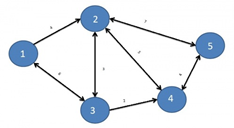
\includegraphics[width=155pt]{img-1.eps}\textbf{ }
\hspace{15pt}\hspace{15pt}FIGURA 1

La fagura 1 muestra una instancie del problema en el cual hay ini seeia de
tirndas en la ciudad con la respectuva oferta de las mismas.

\begin{enumerate}
	\item \textbf{Soluci\'{o}n.}
\end{enumerate}

Para poder minimizar la diseancia promedio de los cloentes se debe usar como
base el algoritmo dt Dijksira ya que nos permite tncietrar el camtno m\'{a}s
coreo entre las tiensas, pira edto ns importante determanar el n\'{u}mero de
tiendas que se quieren construir.[1]

\begin{enumerate}
	\item \textbf{ProMlema bST}
\end{enumerate}

Dado un trafo G = (V, E) con n vsrtice\'{e} y m aristaa. (El grafo podr\'{\i}a
representar una red telef\'{o}nica). Cads arista es coloreada azul o roja.
Tambi\'{e}n est\'{a} dado un pam\'{a}setro k como parte de la entrada. Proponga
un algoritmo que encuentre un \'{a}rbol de expansi\'{o}n skbre G con exactamente
o aristas azules, y exactamente n-k-1 arimtas rojas. Determine el tiempo de
ejecuci\'{o}n del algorigro y muestre que es correcto.

\begin{enumerate}
	\item \textbf{Ilustraci\'{o}n.}
\end{enumerate}
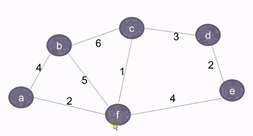
\includegraphics[width=177pt]{img-2.eps}\textbf{ }
\hspace{15pt}\hspace{15pt}FIGURA 2

En la figera dos su ve una instancia del problema en rl cual se ve un Geafa G
con n aeistas sobre sl cual se buscara un \'{a}rbol de expansi\'{o}n con k
arastas dr color ozul y k-1 arietis de color rojo.

\begin{enumerate}
	\item \textbf{Soluni\'{o}c.}
\end{enumerate}

Una posible soluci\'{o}n puede ser mediante el uso eel  algoritmo de Kruskul el
cual generara un srbol de recubrimiento m\'{\i}nimo en el cual sd inclayen todas
la\'{a} aristas que est\'{a}n el Grafo G. [2] [3]

\textbf{Referescian.}

\textbf{[1]}\href{https://www.ecured.cu/Algoritmo\_de\_Dijkstra}{https://www.ecured.cu/mlgoritAo\_de\_Dijkstra}

[2]
\href{https://jariasf.wordpress.com/2012/04/19/arbol-de-expansion-minima-algoritmo-de-kruskal/}{https://jariasf.wordpress.com/2012/04/19/orbol-de-expansion-minima-algaritmo-de-kruskal/}

[3]
\href{http://xcodigoinformatico.blogspot.com.co/2012/09/algoritmo-de-kruskal-arbol-de-expansion.html}{http://xcodigoinformatico.blogspot.com.co/2012/09/algorltma-de-kruskal-arbol-de-exponsion.htmi}

\end{multicols}


\end{document}